% !TeX spellcheck = pl_PL
%%%%%%%%%%%%%%%%%%%%%%%%%%%%%%%%%%%%%%%%%%%
%                                        %
% Szablon pracy dyplomowej inzynierskiej %
% zgodny  z aktualnymi  przepisami  SZJK %
%                                        %
%%%%%%%%%%%%%%%%%%%%%%%%%%%%%%%%%%%%%%%%%%
%                                        %
%  (c) Krzysztof Simiński, 2018-2023     %
%                                        %
%%%%%%%%%%%%%%%%%%%%%%%%%%%%%%%%%%%%%%%%%%
%                                        %
% Najnowsza wersja szablonów jest        %
% podstępna pod adresem                  %
% github.com/ksiminski/polsl-aei-theses  %
%                                        %
%%%%%%%%%%%%%%%%%%%%%%%%%%%%%%%%%%%%%%%%%%
%
%
% Projekt LaTeXowy zapewnia odpowiednie formatowanie pracy,
% zgodnie z wymaganiami Systemu zapewniania jakości kształcenia.
% Proszę nie zmieniać ustawień formatowania (np. fontu,
% marginesów, wytłuszczeń, kursywy itd. ).
%
% Projekt można kompilować na kilka sposobów.
%
% 1. kompilacja pdfLaTeX
%
% pdflatex main
% bibtex   main
% pdflatex main
% pdflatex main
%
%
% 2. kompilacja XeLaTeX
%
% Kompilatacja przy użyciu XeLaTeXa różni się tym, że na stronie
% tytułowej używany jest font Calibri. Wymaga to jego uprzedniego
% zainstalowania.
%
% xelatex main
% bibtex  main
% xelatex main
% xelatex main
%
%
%%%%%%%%%%%%%%%%%%%%%%%%%%%%%%%%%%%%%%%%%%%%%%%%%%%%%
% W przypadku pytań, uwag, proszę pisać na adres:   %
%      krzysztof.siminski(małpa)polsl.pl            %
%%%%%%%%%%%%%%%%%%%%%%%%%%%%%%%%%%%%%%%%%%%%%%%%%%%%%
%
% Chcemy ulepszać szablony LaTeXowe prac dyplomowych.
% Wypełniając ankietę spod poniższego adresu pomogą
% Państwo nam to zrobić. Ankieta jest całkowicie
% anonimowa. Dziękujemy!


% https://docs.google.com/forms/d/e/1FAIpQLScyllVxNKzKFHfILDfdbwC-jvT8YL0RSTFs-s27UGw9CKn-fQ/viewform?usp=sf_link
%
%%%%%%%%%%%%%%%%%%%%%%%%%%%%%%%%%%%%%%%%%%%%%%%%%%%%%%%%%%%%%%%%%%%%%%%%%

%%%%%%%%%%%%%%%%%%%%%%%%%%%%%%%%%%%%%%%%%%%%%%%
%                                             %
% PERSONALIZACJA PRACY – DANE PRACY           %
%                                             %
%%%%%%%%%%%%%%%%%%%%%%%%%%%%%%%%%%%%%%%%%%%%%%%

% Proszę wpisać swoje dane w poniższych definicjach.

% TODO
% dane autora
\newcommand{\FirstNameAuthor}{Aleksandra}
\newcommand{\SurnameAuthor}{Kyc}
\newcommand{\IdAuthor}{296410}   % numer albumu  (bez $\langle$ i $\rangle$)

% drugi autor:
%\newcommand{\FirstNameCoauthor}{Imię}   % Jeżeli jest drugi autor, to tutaj należy podać imię.
%\newcommand{\SurnameCoauthor}{Nazwisko} % Jeżeli jest drugi autor, to tutaj należy podać nazwisko.
%\newcommand{\IdCoauthor}{$\langle$wpisać właściwy$\rangle$}  % numer albumu drugiego autora (bez $\langle$ i $\rangle$)
% Gdy nie ma drugiego autora, należy zostawić poniższe definicje puste, jak poniżej. Gdy jest drugi autor, należy zakomentować te linie.
\newcommand{\FirstNameCoauthor}{} % Jeżeli praca ma tylko jednego autora, to dane drugiego autora zostają puste.
\newcommand{\SurnameCoauthor}{}   % Jeżeli praca ma tylko jednego autora, to dane drugiego autora zostają puste.
\newcommand{\IdCoauthor}{}  % Jeżeli praca ma tylko jednego autora, to dane drugiego autora zostają puste.
%%%%%%%%%%

\newcommand{\Supervisor}{dr hab. inż., prof. PŚ Krzysztof Simiński}     % dane promotora (bez $\langle$ i $\rangle$)
\newcommand{\Title}{Aplikacja mobilna do nauki znaków kanji}           % tytuł pracy po polsku
\newcommand{\TitleAlt}{Mobile application for Kanji learning}                     % thesis title in English
\newcommand{\Program}{Informatyka}            % kierunek studiów  (bez $\langle$ i $\rangle$)
\newcommand{\Specialisation}{Grafika Komputerowa i Oprogramowanie}     % specjalność  (bez $\langle$ i $\rangle$)
\newcommand{\Departament}{Algorytmiki i Oprogramowania }        % katedra promotora  (bez $\langle$ i $\rangle$)

% Jeżeli został wyznaczony promotor pomocniczy lub opiekun, proszę go/ją wpisać ...
%\newcommand{\Consultant}{$\langle$stopień naukowy imię i nazwisko$\rangle$} % dane promotora pomocniczego, opiekuna (bez $\langle$ i $\rangle$)
% ... w przeciwnym razie proszę zostawić puste miejsce jak poniżej:
\newcommand{\Consultant}{} % brak promotowa pomocniczego / opiekuna

% koniec fragmentu do modyfikacji
%%%%%%%%%%%%%%%%%%%%%%%%%%%%%%%%%%%%%%%%%%


%%%%%%%%%%%%%%%%%%%%%%%%%%%%%%%%%%%%%%%%%%%%%%%
%                                             %
% KONIEC PERSONALIZACJI PRACY                 %
%                                             %
%%%%%%%%%%%%%%%%%%%%%%%%%%%%%%%%%%%%%%%%%%%%%%%

%%%%%%%%%%%%%%%%%%%%%%%%%%%%%%%%%%%%%%%%


%%%%%%%%%%%%%%%%%%%%%%%%%%%%%%%%%%%%%%%%%%%%%%%
%                                             %
% PROSZĘ NIE MODYFIKOWAĆ PONIŻSZYCH USTAWIEŃ! %
%                                             %
%%%%%%%%%%%%%%%%%%%%%%%%%%%%%%%%%%%%%%%%%%%%%%%



\documentclass[a4paper,twoside,12pt]{book}
\usepackage[utf8]{inputenc}                                      
\usepackage[T1]{fontenc}  
\usepackage{amsmath,amsfonts,amssymb,amsthm}
\usepackage[british,polish]{babel} 
\usepackage{indentfirst}
\usepackage{xurl}
\usepackage{xstring}
\usepackage{ifthen}


\usepackage{ifxetex}

\ifxetex
	\usepackage{fontspec}
	\defaultfontfeatures{Mapping=tex—text} % to support TeX conventions like ``——-''
	\usepackage{xunicode} % Unicode support for LaTeX character names (accents, European chars, etc)
	\usepackage{xltxtra} % Extra customizations for XeLaTeX
\else
	\usepackage{lmodern}
\fi



\usepackage[margin=2.5cm]{geometry}
\usepackage{graphicx} 
\usepackage{hyperref}
\usepackage{booktabs}
\usepackage{tikz}
\usepackage{pgfplots}
\usepackage{mathtools}
\usepackage{geometry}
\usepackage{subcaption}   % subfigures
\usepackage[page]{appendix} % toc,
\renewcommand{\appendixtocname}{Dodatki}
\renewcommand{\appendixpagename}{Dodatki}
\renewcommand{\appendixname}{Dodatek}

\usepackage{csquotes}
\usepackage[natbib=true,backend=bibtex,maxbibnames=99]{biblatex}  % kompilacja bibliografii BibTeXem
%\usepackage[natbib=true,backend=biber,maxbibnames=99]{biblatex}  % kompilacja bibliografii Biberem
\bibliography{biblio}

\usepackage{ifmtarg}   % empty commands  

\usepackage{setspace}
\onehalfspacing


\frenchspacing

%%%%%%%%%%%%%%%%%%%%%%%%%%%%%%%%%%
% środowiska dla definicji, twierdzenia, przykładu
\usepackage{amsthm}

\newtheorem{Definition}{Definicja}
\newtheorem{Example}{Przykład}
\newtheorem{Theorem}{Twierdzenie}
%%%%%%%%%%%%%%%%%%%%%%%%%%%%%%%%%%

%%%% TODO LIST GENERATOR %%%%%%%%%

\usepackage{color}
\definecolor{brickred}      {cmyk}{0   , 0.89, 0.94, 0.28}

\makeatletter \newcommand \kslistofremarks{\section*{Uwagi} \@starttoc{rks}}
  \newcommand\l@uwagas[2]
    {\par\noindent \textbf{#2:} %\parbox{10cm}
{#1}\par} \makeatother


\newcommand{\ksremark}[1]{%
{%\marginpar{\textdbend}
{\color{brickred}{[#1]}}}%
\addcontentsline{rks}{uwagas}{\protect{#1}}%
}

\newcommand{\comma}{\ksremark{przecinek}}
\newcommand{\nocomma}{\ksremark{bez przecinka}}
\newcommand{\styl}{\ksremark{styl}}
\newcommand{\ortografia}{\ksremark{ortografia}}
\newcommand{\fleksja}{\ksremark{fleksja}}
\newcommand{\pauza}{\ksremark{pauza `--', nie dywiz `-'}}
\newcommand{\kolokwializm}{\ksremark{kolokwializm}}
\newcommand{\cudzyslowy}{\ksremark{,,polskie cudzysłowy''}}

%%%%%%%%%%%%%% END OF TODO LIST GENERATOR %%%%%%%%%%%

\newcommand{\printCoauthor}{%		
    \StrLen{\FirstNameCoauthor}[\FNCoALen]
    \ifthenelse{\FNCoALen > 0}%
    {%
		{\large\bfseries\Coauthor\par}
	
		{\normalsize\bfseries \LeftId: \IdCoauthor\par}
    }%
    {}
} 

%%%%%%%%%%%%%%%%%%%%%
\newcommand{\autor}{%		
    \StrLen{\FirstNameCoauthor}[\FNCoALenXX]
    \ifthenelse{\FNCoALenXX > 0}%
    {\FirstNameAuthor\ \SurnameAuthor, \FirstNameCoauthor\ \SurnameCoauthor}%
	{\FirstNameAuthor\ \SurnameAuthor}%
}
%%%%%%%%%%%%%%%%%%%%%

\StrLen{\FirstNameCoauthor}[\FNCoALen]
\ifthenelse{\FNCoALen > 0}%
{%
\author{\FirstNameAuthor\ \SurnameAuthor, \FirstNameCoauthor\ \SurnameCoauthor}
}%
{%
\author{\FirstNameAuthor\ \SurnameAuthor}
}%

%%%%%%%%%%%% ZYWA PAGINA %%%%%%%%%%%%%%%
% brak kapitalizacji zywej paginy
\usepackage{fancyhdr}
\pagestyle{fancy}
\fancyhf{}
\fancyhead[LO]{\nouppercase{\it\rightmark}}
\fancyhead[RE]{\nouppercase{\it\leftmark}}
\fancyhead[LE,RO]{\it\thepage}


\fancypagestyle{tylkoNumeryStron}{%
   \fancyhf{} 
   \fancyhead[LE,RO]{\it\thepage}
}

\fancypagestyle{bezNumeracji}{%
   \fancyhf{} 
   \fancyhead[LE,RO]{}
}


\fancypagestyle{NumeryStronNazwyRozdzialow}{%
   \fancyhf{} 
   \fancyhead[LE]{\nouppercase{\autor}}
   \fancyhead[RO]{\nouppercase{\leftmark}} 
   \fancyfoot[CE, CO]{\thepage}
}


%%%%%%%%%%%%% OBCE WTRETY  
\newcommand{\obcy}[1]{\emph{#1}}
\newcommand{\english}[1]{{\selectlanguage{british}\obcy{#1}}}
%%%%%%%%%%%%%%%%%%%%%%%%%%%%%

% polskie oznaczenia funkcji matematycznych
\renewcommand{\tan}{\operatorname {tg}}
\renewcommand{\log}{\operatorname {lg}}

% jeszcze jakies drobiazgi

\newcounter{stronyPozaNumeracja}

%%%%%%%%%%%%%%%%%%%%%%%%%%% 
\newcommand{\printOpiekun}[1]{%		

    \StrLen{\Consultant}[\mystringlen]
    \ifthenelse{\mystringlen > 0}%
    {%
       {\large{\bfseries OPIEKUN, PROMOTOR POMOCNICZY}\par}
       
       {\large{\bfseries \Consultant}\par}
    }%
    {}
} 
%
%%%%%%%%%%%%%%%%%%%%%%%%%%%%%%%%%%%%%%%%%%%%%%
 
% Proszę nie modyfikować poniższych definicji!
\newcommand{\Author}{\FirstNameAuthor\ \MakeUppercase{\SurnameAuthor}} 
\newcommand{\Coauthor}{\FirstNameCoauthor\ \MakeUppercase{\SurnameCoauthor}}
\newcommand{\Type}{PROJEKT INŻYNIERSKI}
\newcommand{\Faculty}{Wydział Automatyki, Elektroniki i Informatyki} 
\newcommand{\Polsl}{Politechnika Śląska}
\newcommand{\Logo}{politechnika_sl_logo_bw_pion_pl.pdf}
\newcommand{\LeftId}{Nr albumu}
\newcommand{\LeftProgram}{Kierunek}
\newcommand{\LeftSpecialisation}{Specjalność}
\newcommand{\LeftSUPERVISOR}{PROWADZĄCY PRACĘ}
\newcommand{\LeftDEPARTMENT}{KATEDRA}
%%%%%%%%%%%%%%%%%%%%%%%%%%%%%%%%%%%%%%%%%%%%%%

%%%%%%%%%%%%%%%%%%%%%%%%%%%%%%%%%%%%%%%%%%%%%%%
%                                             %
% KONIEC USTAWIEŃ                             %
%                                             %
%%%%%%%%%%%%%%%%%%%%%%%%%%%%%%%%%%%%%%%%%%%%%%%




%%%%%%%%%%%%%%%%%%%%%%%%%%%%%%%%%%%%%%%%%%%%%%%
%                                             %
% MOJE PAKIETY, USTAWIENIA ITD                %
%                                             %
%%%%%%%%%%%%%%%%%%%%%%%%%%%%%%%%%%%%%%%%%%%%%%%

% Tutaj proszę umieszczać swoje pakiety, makra, ustawienia itd.

\usepackage{graphicx}
\graphicspath{ {../Diagrams/} }
\usepackage{float}
%\newcommand{\japanese}[1]{{\selectlanguage{japanese}\obcy{#1}}} 
 
%%%%%%%%%%%%%%%%%%%%%%%%%%%%%%%%%%%%%%%%%%%%%%%%%%%%%%%%%%%%%%%%%%%%%
% listingi i fragmentu kodu źródłowego 
% pakiet: listings lub minted
% % % % % % % % % % % % % % % % % % % % % % % % % % % % % % % % % % % 

% biblioteka listings
\usepackage{listings}
\lstset{%
morekeywords={string,exception,std,vector},% słowa kluczowe rozpoznawane przez pakiet listings
language=C++,% C, Matlab, Python, SQL, TeX, XML, bash, ... – vide https://www.ctan.org/pkg/listings
commentstyle=\textit,%
identifierstyle=\textsf,%
keywordstyle=\sffamily\bfseries, %\texttt, %
%captionpos=b,%
tabsize=3,%
frame=lines,%
numbers=left,%
numberstyle=\tiny,%
numbersep=5pt,%
breaklines=true,%
escapeinside={@*}{*@},%
}

% % % % % % % % % % % % % % % % % % % % % % % % % % % % % % % % % % % 
% pakiet minted
%\usepackage{minted}

% pakiet wymaga specjalnego kompilowania:
% pdflatex -shell-escape main.tex
% xelatex  -shell-escape main.tex

%\usepackage[chapter]{minted} % [section]
%%\usemintedstyle{bw}   % czarno-białe kody 
%
%\setminted % https://ctan.org/pkg/minted
%{
%%fontsize=\normalsize,%\footnotesize,
%%captionpos=b,%
%tabsize=3,%
%frame=lines,%
%framesep=2mm,
%numbers=left,%
%numbersep=5pt,%
%breaklines=true,%
%escapeinside=@@,%
%}

%%%%%%%%%%%%%%%%%%%%%%%%%%%%%%%%%%%%%%%%%%%%%%%%%%%%%%%%%%%%%%%%%%%%%



%%%%%%%%%%%%%%%%%%%%%%%%%%%%%%%%%%%%%%%%%%%%%%%
%                                             %
% KONIEC MOICH USTAWIEŃ                       %
%                                             %
%%%%%%%%%%%%%%%%%%%%%%%%%%%%%%%%%%%%%%%%%%%%%%%



%%%%%%%%%%%%%%%%%%%%%%%%%%%%%%%%%%%%%%%%


\begin{document}
\kslistofremarks

\frontmatter

%%%%%%%%%%%%%%%%%%%%%%%%%%%%%%%%%%%%%%%%%%%%%%%
%                                             %
% PROSZĘ NIE MODYFIKOWAĆ STRONY TYTUŁOWEJ!    %
%                                             %
%%%%%%%%%%%%%%%%%%%%%%%%%%%%%%%%%%%%%%%%%%%%%%%


%%%%%%%%%%%%%%%%%%  STRONA TYTUŁOWA %%%%%%%%%%%%%%%%%%%
\pagestyle{empty}
{
	\newgeometry{top=1.5cm,%
	             bottom=2.5cm,%
	             left=3cm,
	             right=2.5cm}
 
	\ifxetex 
	  \begingroup
	  \setsansfont{Calibri}
	   
	\fi 
	 \sffamily
	\begin{center}
	\includegraphics[width=50mm]{\Logo}
	 
	
	{\Large\bfseries\Type\par}
	
	\vfill  \vfill  
			 
	{\large\Title\par}
	
	\vfill  
		
	{\large\bfseries\Author\par}
	
	{\normalsize\bfseries \LeftId: \IdAuthor}

	\printCoauthor
	
	\vfill  		
 
	{\large{\bfseries \LeftProgram:} \Program\par} 
	
	{\large{\bfseries \LeftSpecialisation:} \Specialisation\par} 
	 		
	\vfill  \vfill 	\vfill 	\vfill 	\vfill 	\vfill 	\vfill  
	 
	{\large{\bfseries \LeftSUPERVISOR}\par}
	
	{\large{\bfseries \Supervisor}\par}
				
	{\large{\bfseries \LeftDEPARTMENT\ \Departament} \par}
		
	{\large{\bfseries \Faculty}\par}
		
	\vfill  \vfill  

    	
    \printOpiekun{\Consultant}
    
	\vfill  \vfill  
		
    {\large\bfseries  Katowice \the\year}

   \end{center}	
       \ifxetex 
       	  \endgroup
       \fi
	\restoregeometry
}
  
%%%%%%%%%%%%%%%%%%%%%%%%%%%%%%%%%%%%%%%%%%%%%%%
%                                             %
% KONIEC STRONY TYTUŁOWEJ                     %
%                                             %
%%%%%%%%%%%%%%%%%%%%%%%%%%%%%%%%%%%%%%%%%%%%%%%  


\cleardoublepage

\rmfamily\normalfont
\pagestyle{empty}


%%% No to zaczynamy pisać pracę :-) %%%%

% TODO
\subsubsection*{Tytuł pracy} 
\Title

\subsubsection*{Streszczenie}  
(Streszczenie pracy – odpowiednie pole w systemie APD powinno zawierać kopię tego streszczenia.)

\subsubsection*{Słowa kluczowe} 
(2-5 slow (fraz) kluczowych, oddzielonych przecinkami)

\subsubsection*{Thesis title} 
\begin{otherlanguage}{british}
\TitleAlt
\end{otherlanguage}

\subsubsection*{Abstract} 
\begin{otherlanguage}{british}
(Thesis abstract – to be copied into an appropriate field during an electronic submission – in English.)
\end{otherlanguage}
\subsubsection*{Key words}  
\begin{otherlanguage}{british}
(2-5 keywords, separated by commas)
\end{otherlanguage}



%%%%%%%%%%%%%%%%%% SPIS TRESCI %%%%%%%%%%%%%%%%%%%%%%
% Add \thispagestyle{empty} to the toc file (main.toc), because \pagestyle{empty} doesn't work if the TOC has multiple pages
\addtocontents{toc}{\protect\thispagestyle{empty}}
\tableofcontents

%%%%%%%%%%%%%%%%%%%%%%%%%%%%%%%%%%%%%%%%%%%%%%%%%%%%%
\setcounter{stronyPozaNumeracja}{\value{page}}
\mainmatter
\pagestyle{empty}

\cleardoublepage

\pagestyle{NumeryStronNazwyRozdzialow}

%%%%%%%%%%%%%% wlasciwa tresc pracy %%%%%%%%%%%%%%%%%

% TODO
\chapter{Wstęp}
\label{ch:wstep}

\ksremark{Wstępem zajmiemy się na końcu.}
Aby wyjaśnić cel tej pracy inżynierskiej, należy wspomnieć o kilku ważnych pojęciach związanych z językiem japońskim i jego nauką. Kanji razem z sylabariuszami hiragana i katakana oraz znanymi nam cyframi arabskimi i alfabetem romańskim tworzą całość japońskiego alfabetu. Są to znaki logograficzne, co oznacza że przeciwnie do alfabetów składających się z głosek, każdy znak oznacza jakieś pojęcie. Kompleksowa lista wszystkich kanji nie istnieje, jednak ich liczbę szacuje się na około czterdziestu tysięcy. Jest to ogromna liczba, na którą składa się wiele znaków przestarzałych lub bardzo rzadko używanych. Zamiast niej częstym wskaźnikiem płynności językowej w kontekście kanji jest pojęcie \textit{jōyō kanji}, które oznacza zestaw znaków wymagany przez japoński system edukacji. Po ukończeniu szkoły średniej Japończyk posługuje się 2136 znakami kanji. Podobna liczba potrzebna jest, aby zdać test znajomości języka japońskiego dla obcokrajowców (jap. \textit{Nihongo nōryoku shiken}) na najwyższym poziomie oraz zawiera się w około 98 procentach tekstu pisanego.

Zaznajomienie się ze znakami kanji to nieodłączna część nauki języka japońskiego. Co prawda uparty uczeń może zaprzestać na nauce gramatyki, wymowy i zromanizowanego zapisu \textit{rōmaji}, ale poskutkuje to wątpliwą płynnością językową, gdyż nie będzie w stanie przeczytać nawet książki lub restauracyjnego menu. Dla początkującego tak duża ilość materiału może być odrzucająca, dlatego na rynku pojawiło się wiele rozwiązań, które pomagają użytkownikowi w nauce kanji. Jednym z takich rozwiązań jest aplikacja mobilna opracowana na rzecz tej pracy inżynierskiej.

Celem pracy jest stworzenie rozwiązania wspomagającego ucznia w nauce kanji jako aplikacji mobilnej. Program powinien posiadać skuteczny tryb nauczania, który potrafi dostosować się do poziomu ucznia. Jako że kluczowa dla zapamiętaniu tak dużej liczby znaków systematyczność jest trudna do osiągnięcia, aplikacja powinna motywować do kolejnych podejść i dostarczać różnorodne ćwiczenia. Ważnym zagadnieniem w rozwiązaniu tego rodzaju jest też odpowiedni rozrzut pytań w czasie. Ta praca stara się wziąć pod uwagę fakt, że niektóre znaki mogą przyjść uczniowi łatwo, a inne trudno i należy odpowiednio dostosować algorytm dostarczający zadania do wykonania.

Rozwiązanie opisane w tej pracy to obok aplikacji mobilnej system wspomagający jej działanie. Na zakres pracy składa się sama aplikacja, baza danych dotyczących użytkowników oraz panel administracyjny jako aplikacja webowa. Rozwiązanie obsługuje trzy rodzaje użytkowników, którymi są uczeń, nauczyciel i administrator. Uczeń to użytkownik korzystający z takich funkcjonalności aplikacji jak przeglądanie słownika kanji, tworzenie zestawów znaków oraz tryb nauki. Aby ułatwić wybór znaków do nauki, aplikacja jest wyposażona w predefiniowane zestawy, które odpowiadają poziomom egzaminu językowego lub kolejnym klasom w japońskim szkolnictwie. Nauczyciel to użytkownik, który może tworzyć grupy uczniów, zadawać im zadania domowe i sprawdzać ich postępy. Takie rozwiązanie ma pomagać w nauce w trybie zajęć grupowych, gdzie nauczyciel spotyka się z uczniami kilka razy w miesiącu i chce motywować do dalszej pracy w domu. 

% TODO
\chapter{Analiza tematu}

\section{Nauka języków obcych wspomagana komputerowo}
%\begin{itemize}
%\item sformułowanie problemu
%\item osadzenie tematu w kontekśceeie aktualnego stanu wiedzy (\english{state of the art}) o poruszanym problemie
%\item  studia literaturowe e e%\cite{bib:artykul,bib:ksiazka,bib:konferencja,bib:internet} -  opis znanych rozwiązań (także opisanych naukowo, jeżeli problem jest poruszany w publikacjach naukowych), algorytmów, 
%\end{itemize}

%sformulowanie problemu 

%- jak uczyc sie ogolnie i za pomoca komputera: research, spaced repetition, computer %assisted learning. mozna nn tam wrzucic ale w sumie czy to ma az takie znaczenie?
%- jak uczyc sie kanji: rozne aspekty. wyglad, pisanie(stroke order),  czytania, %zlozenia, zdania. Podzial na zestawy: w jakiej kolejnosci nauka.

%osadzenie w kontekscie aktualnego stanu wiedzy

%- globalny computer assisted learning, jego wady i zalety
%- jak wygladaja konkretnie apki do nauki j.j i kanji

Próby usystematyzowania nauki, szczególnie gdy materiał wymaga od nas więcej zapamiętywania niż analizy problemów, są naturalnie występującym skutkiem konieczności żmudnego, wielokrotnego powtarzania. Uczniowie wykazujący się większym sprytem niż pracowitością szukają drogi na skróty, aby tę samą ilość materiału przyswoić w krótszym czasie. Tak powstały pierwsze metody technik zapamiętywania, na przykład fiszki, czyli niewielkie kawałki papieru z pytaniem na jednej stronie i odpowiedzią na drugiej. Taki system pozwala na kompaktowe przechowywanie materiału, co pozwala uczyć się również w krótkich chwilach czasu i daleko od domu, na przykład w autobusie. 

Dziennikarz Sebastian Leitner w 1972 wymyślił sposób na dalsze usprawnienie nauki za pomocą fiszek \cite{bib:internetLeitner}. W metodzie Leitnera fiszki są podzielone na grupy względem tego, jak dobrze uczeń zna dany materiał. Jeżeli uczeń odpowie dobrze na dane pytanie, przenosi fiszkę do następnego pudełka. Jeśli odpowie źle, fiszka wraca na początek. Grupy różni to, jak często użytkownik jest zobowiązany powtarzać dany materiał. Im materiał lepiej znany, tym rzadziej uczeń musi go powtarzać. 

\begin{figure}
\centering
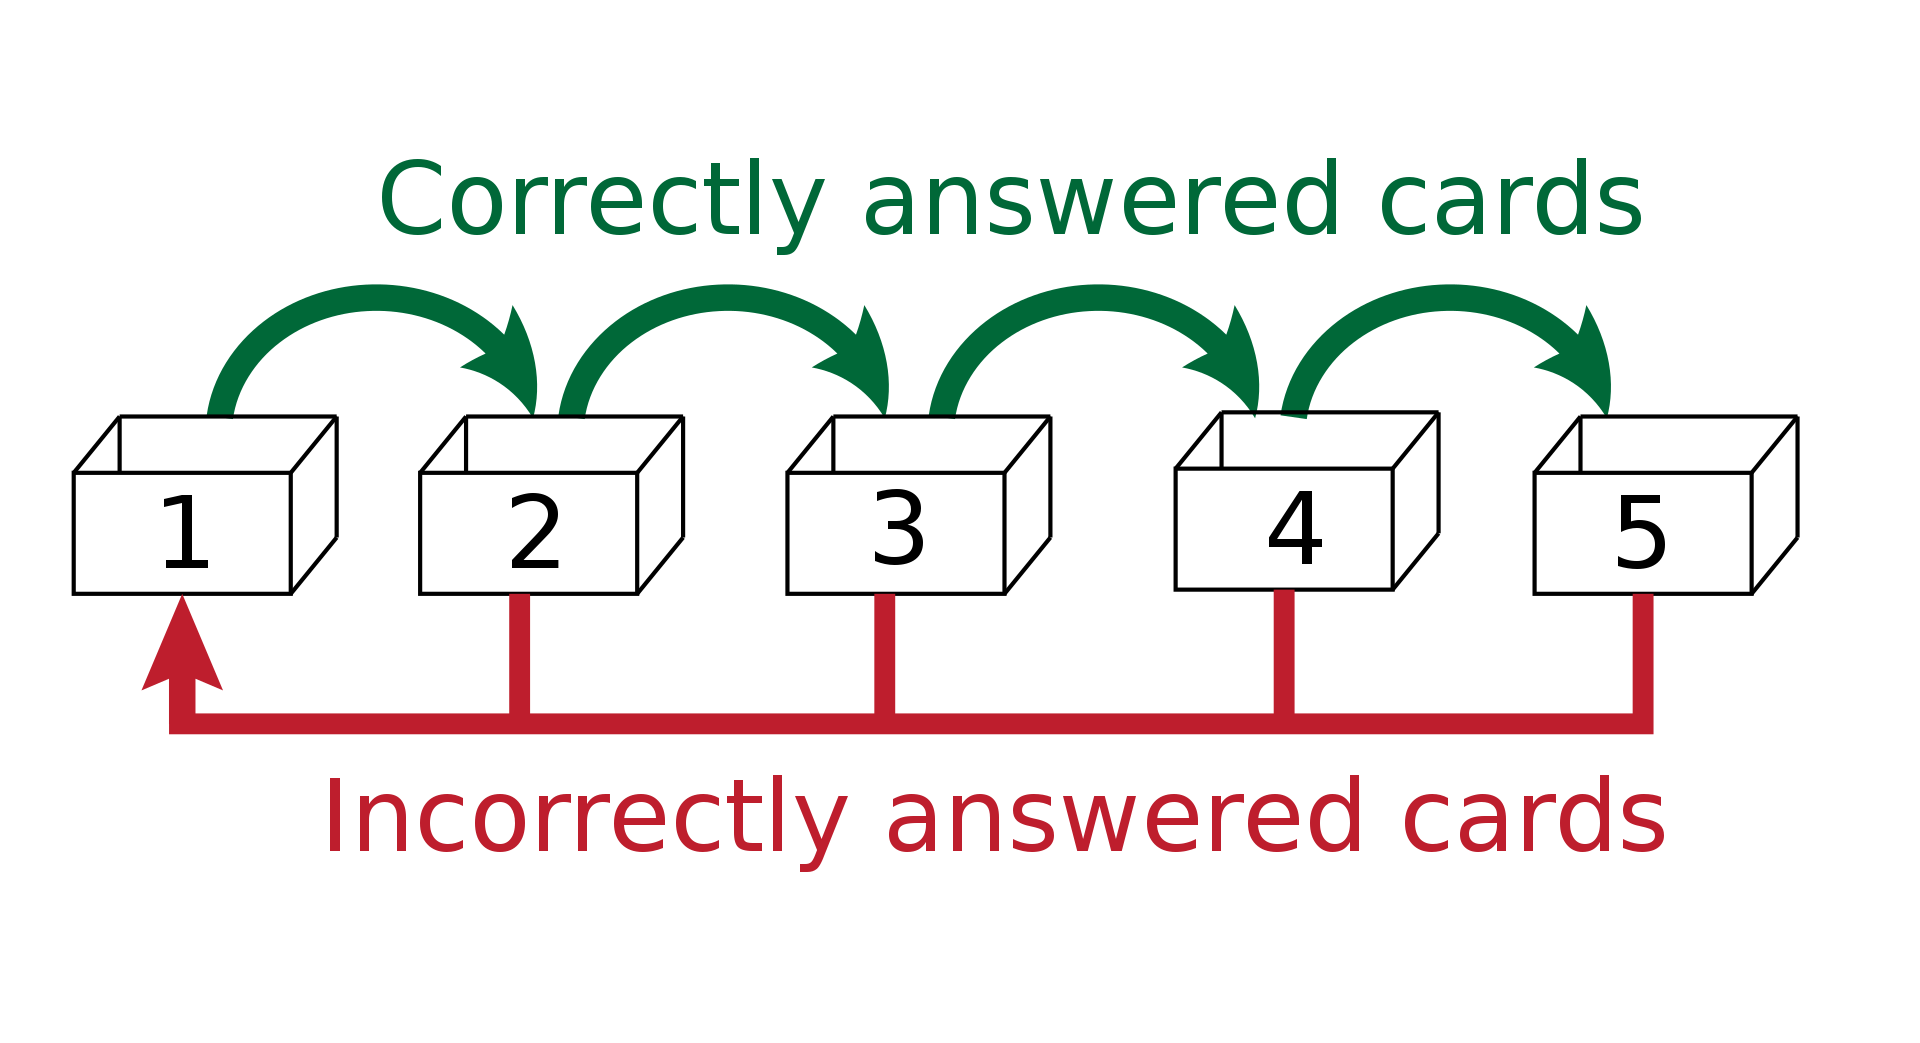
\includegraphics[width=0.5\textwidth]{leitner_system}
\caption{Ilustracja reprezentująca system wykorzystujący fiszki.}
\label{fig:etykieta-rysunku1}
\end{figure}
%https://en.wikipedia.org/wiki/Spaced_repetition#/media/File:Leitner_system_alternative.svg

Sposób Leitnera, mimo że skuteczny, jest żmudny do implementacji. Uczeń musi napisać ręcznie wszystkie fiszki, zrobić lub zakupić kilka pudełek o podobnym rozmiarze, rozkladać ten obszerny zestaw za każdym razem, gdy chce powtórzyć materiał. Tym samym traci mobilność, która jest dużą zaletą fiszek. W tym miejscu z pomocą przychodzi nauka języków wspomagana komputerowo (ang. Computer-Assisted Language Learning, CALL). Jest to rozwijana \citep{bib:konferencjaCALLhistory} od lat pięćdziesiątych dwudziestego wieku dziedzina wykorzystująca komputery do poprawiania umiejętności językowych. Ten sposób podejścia do problemu zrzuca z barków uczniów część problemów z tworzeniem fiszek, a wraz z popularyzacją urządzeń takich jak smartfony czy tablety zwraca mobilność nauki. 

Algorytm powtórek w interwałach (eng. \textit{spaced repetition}), którego papierową implementacją jest wyżej wspomniany system Leitnera, został poddany wielokrotnym badaniom \cite{bib:artykulAlzheimer} \cite{bib:artykulSpaced}. Wskazują one nie tylko na poprawę jakości zapamiętywania danego materiału, ale też na ogólną poprawę pamięci, szczególnie u osób chorujących na chorobę Alzheimera lub inne schorzenia związane z pogorszeniem umiejętności zapamiętywania \cite{bib:artykulAlzheimer}. Metoda powtórek w interwałach jest szczególnie użyteczna w nauce słownictwa języków obcych. Jest to spowodowane faktem, że informacje do przyswojenia są liczne, lecz małe. Tę samą zasadę można wykorzystać przy nauce znaków kanji. 

Analiza rozwiązań dostępnych na rynku i badań wskazuje na komercyjny i naukowy sukces metody \textit{spaced repetition}. To zdroworozsądkowe podejście ma realny wpływ na szybkość i jakość przyswajania wiedzy. Przez ostatnie kilkadziesiąt lat próbowano udoskonalić ten względnie prosty algorytm z użyciem np. metod sztucznej inteligencji do wyliczania interwałów \cite{bib:internetNN}. Takie podejście ma mieszane rezultaty, nie jest jasne jak realny jest wpływ optymalizacji długości interwału na jakość nauki \cite[rozdział 6]{bib:ksiazkaEssays}.

\section{Analiza rozwiązań dostępnych na rynku}

Aktualnie formą nauczania języków wspomaganą komputerowo cieszącą się szerokim zainteresowaniem jest jej poddziedzina, czyli nauczanie języków obcych wspomagane przez urządzenia mobilne (ang. Mobile-Assisted Language Learning, MALL) \cite{bib:artykulDuolingo}. Największą popularnością  \cite{bib:internetDuolingo} \cite{bib:artykulDuolingo} cieszy się aplikacja \href{https://pl.duolingo.com/}{Duolingo}, która umożliwia naukę pokaźniej listy języków (aż czterdziestu trzech na czas pisania tej pracy) z urządzenia mobilnego lub strony internetowej. Jednym z powodów dobrego przyjęcia Duolingo przez uczniów języków obcych jest podejście bogate w gry i zabawy, motywujące użytkownika przez punkty, nagrody i rankingi \cite{bib:artykulDuolingo}. Aplikacja nie wymaga od użytkownika dużego zaangażowania. Tworzenie własnych zestawów fiszek nie jest konieczne, wystarczy codziennie wykonać kilkanaście zadań wygenerowanych przez system. 

Innym, bardziej angażującym użytkownika programem chętnie wykorzystywanym do nauki jest \href{https://apps.ankiweb.net/}{Anki}. Jest to aplikacja oferująca większą możliwość dostosowania jej do własnych potrzeb, z tego powodu nie jest ograniczona do nauki języków obcych. Użytkownik ma możliwość stworzenie własnego zestawu do nauki złożonego z fiszek, który jest później przyswajany w interwałach zgodnie z zasadą \textit{spaced repetition}. Zaletą Anki jest opcja eksportowania i dzielenia się zestawami między użytkownikami. 

Wyżej wspomniane programy są często używane przez uczniów języka japońskiego i znaków kanji, jednak nie są wyspecjalizowane pod ich potrzeby. Przykładem aplikacji dostosowanej do amatorów japońskiego alfabetu jest \href{https://www.wanikani.com/}{WaniKani}. Ta aplikacja webowa i mobilna obiecuje uczniom nauczenie się 2000 znaków kanji i 6000 słów w nieco dłużej niż rok. Używa metody \textit{spaced repetition} w swojej implementacji ustrukturyzowanego kursu, który jest przeznaczony dla początkujących i pozwala rozwinąć się do biegłego posługiwania się kanji. Aplikacja jest gorzej dostosowana do uczniów o zaawansowanym lub średniozaawansowanym poziomie, ponieważ nie da się dopasować jej pod własne potrzeby językowe. 

\section{Nauka języka japońskiego i znaków kanji}

Ważną kwestią przy nauce kanji, zarówno metodami tradycyjnymi jak i z wykorzystaniem komputerowego wspomagania, jest podejście do przyswajanego materiału. Najważniejszą i obowiązkową kwestią jest zapamiętanie wyglądu i pisowni znaku. Aby wspomóc ten proces, można użyć wskazówek mnemonicznych, czyli pewnego skojarzenia między znaczeniem znaku a jego wyglądem.
%obrazek z mnemonika
Kolejną wskazówką do nauki mogą być klucze, czyli elementy znaku dzielące ich zbiór na podkategorie. Ten podział został stworzony na potrzeby słowników i charakteryzuje znaki na podstawie ich najważniejszgo elementu (podznaku). 
%obrazek?

Wraz z opanowaniem pisowni należy zaznajomić się z czytaniem chińskim (jap. \textit{onyōmi}) i natywnym japońskim (jap. \textit{kunyōmi}). Na nieszczęście uczniów języka japońskiego znaki kanji nie są czytane jednoznacznie i większość z nich ma przynajmniej wyżej wspomniane dwa czytania (wiele z nich ma kilka w ramach \textit{onyōmi} lub \textit{kunyōmi}). Aby urozmaicić naukę czytania znaków kanji można połączyć ją z nauką słów, w których ów znak występuje. Takie podejście wzbogaca zasób słownictwa ucznia i ułatwia zapamiętanie czytań danego znaku przez różnorodne przykłady. Kolejnym możliwym sposobem na połączenie nauki znaków z nauką ogólnie rozumianego języka japońskiego jest załączenie ćwiczeń zawierających całe zdania. Umożliwi to użytkownikom o bardziej zaawansowanym poziomie powtarzać różne znaki w jednym ćwiczeniu oraz rozwinie ich ogólne umiejętności językowe. 

Inną kwestią, często lekceważoną przez samouków, jest kolejność stawiania kresek przy pisaniu znaku. Ten sam znak w teorii może w praktyce wyglądać zupełnie inaczej, jeżeli nieumiejętnie postawimy kolejne linie, z których się składa. Dlatego istotnym jest, żeby w swoją naukę wkomponować dużo pisania ręcznie, nawet jeśli w naszych czasach jest to coraz mniej popularne. Na wprost użytkownikom wychodzą tutaj też aplikacje, które umożliwiają ćwiczenie pisania przez na przykład rysowanie na ekranie. Uważnie wodząc palec lub długopis po ekranie według instrukcji można wyrobić dobre nawyki, które potem należy utrwalić na kartce.

Podobnie jak inne języki, japoński posiada swój własny system egzaminów przeznaczonych dla obcokrajowców. Egzaminy JLPT \textit{(ang. Japanese Language Proficiency Test)} wydzielają pewne poziomy, które określają umiejętności językowe ucznia. W języku japońskim te poziomy oznacza się literą N oraz cyfrą od 1 do 5, gdzie N5 to najniższy, a N1 najbardziej biegły. Do zdania każdego z tych egzaminów potrzebny jest rosnący z poziomu na poziom zasób kanji. Zaczynając od niewielkich liczb jak około sto dla N5 i trzysta dla N4, kończymy na ponad dwu tysiącach dla pełnej biegłości w pisaniu i czytaniu według egzaminatorów.

Podział znaków kanji według trudności wygląda inaczej dla rodzimych mieszkańców Japoni. Jest on ułożony względem systemu szkolnictwa publicznego, podzielony na klasy w których uczniowie poznają dane znaki. Do zestawu dwu tysięcy znaków wymaganych w szkole, czyli \textit{jōyō kanji} dochodzi 846 znaków \textit{jinmeiyō}, które są używane tylko w imionach i nazwiskach.
%%%%%%%%%%%%%%%%%%%%%%%%


% TODO
\chapter{Wymagania i narzędzia}
\label{ch:wymagania-i-narzedzia}

\begin{itemize}
\item wymagania funkcjonalne i niefunkcjonalne
\label{id:tab:wyniki}
\begin{table}[]
\centering
\begin{tabular}{ll}
Przypadek użycia & Priorytet \\
    &           \\
                 &           \\
                 &          
\end{tabular}
\end{table}

\item przypadki użycia (diagramy UML) -- dla prac, w których mają zastosowanie
\begin{figure}
\centering
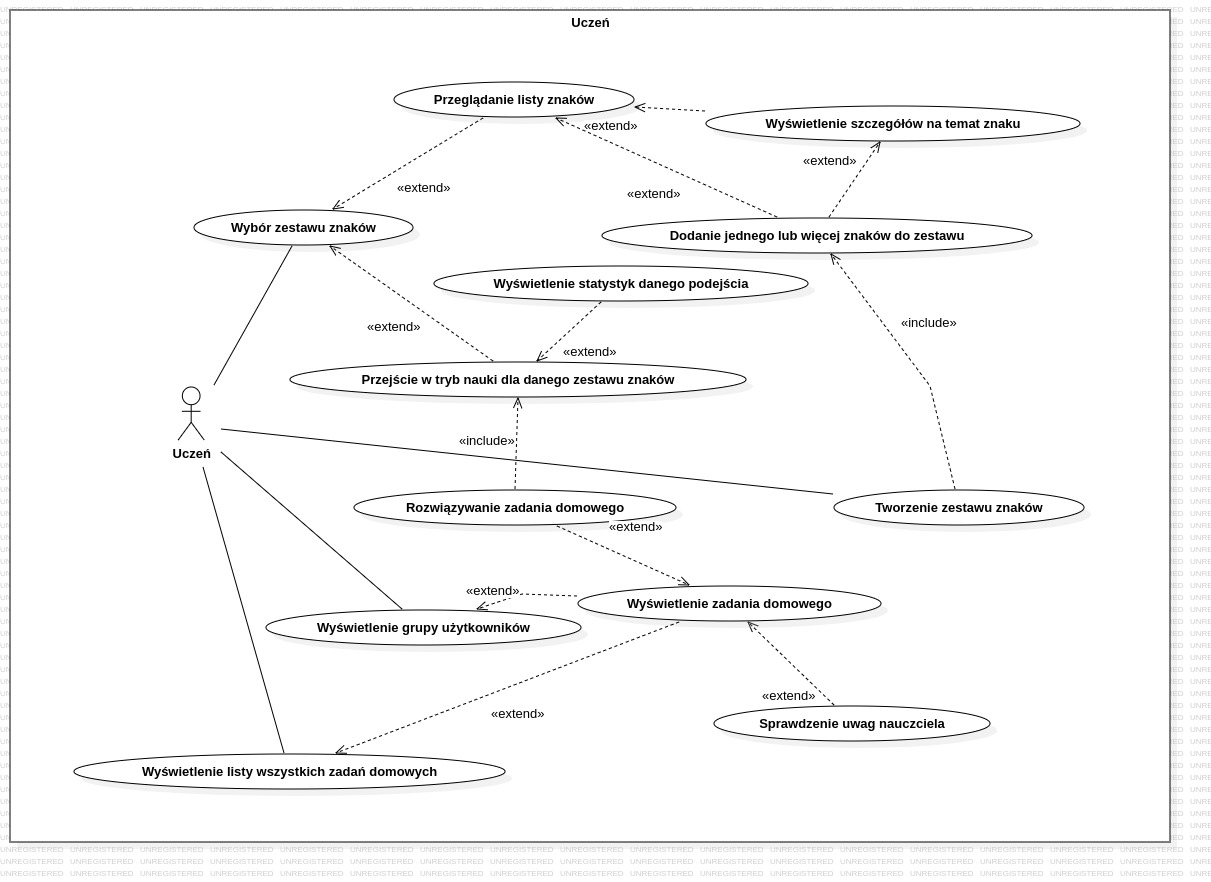
\includegraphics[width=\textwidth]{Uczen}
\caption{Podpis rysunku zawsze pod rysunkiem.}
\label{fig:etykieta-rysunku}
\end{figure}
\begin{figure}
\centering
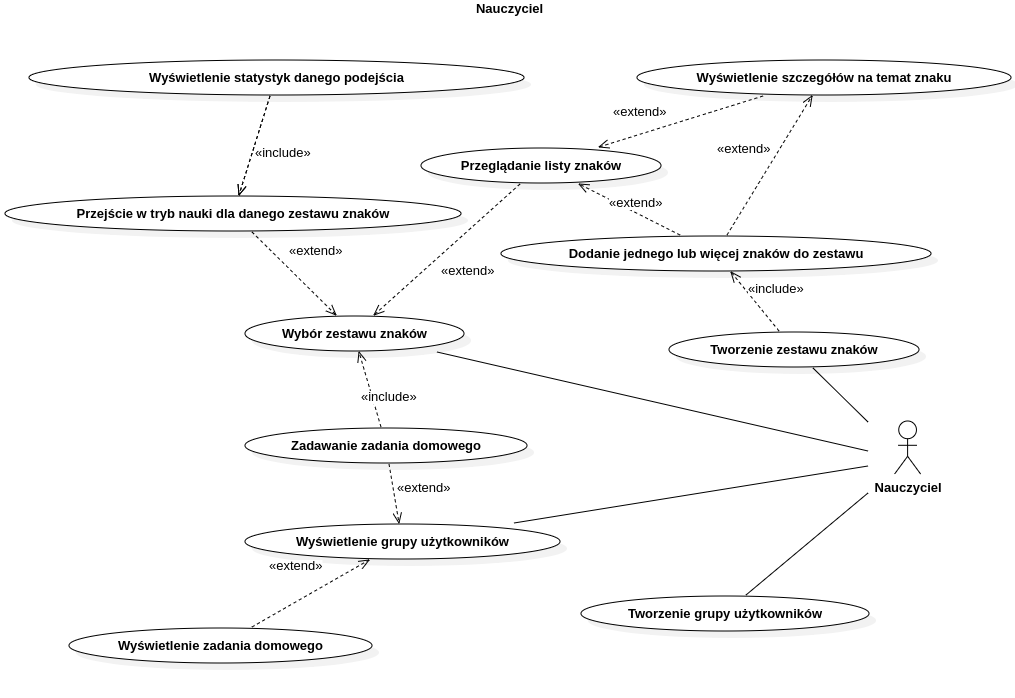
\includegraphics[width=\textwidth]{Nauczyciel}
\caption{Podpis rysunku zawsze pod rysunkiem.}
\label{fig:etykieta-rysunku}
\end{figure}
\begin{figure}
\centering
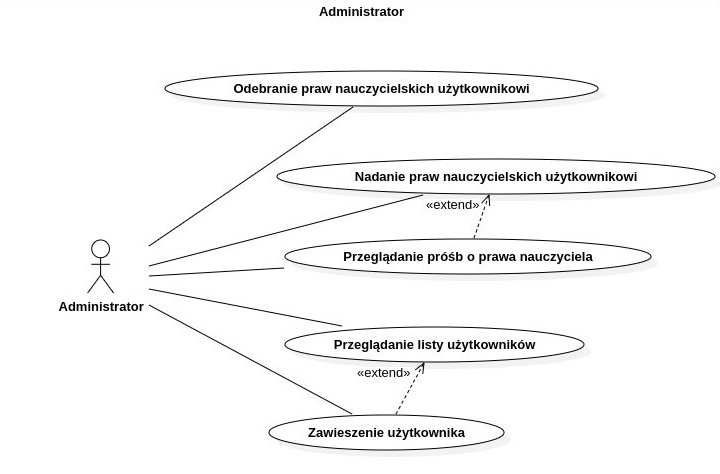
\includegraphics[width=\textwidth]{Admin}
\caption{Podpis rysunku zawsze pod rysunkiem.}
\label{fig:etykieta-rysunku}
\end{figure}
\begin{figure}
\centering
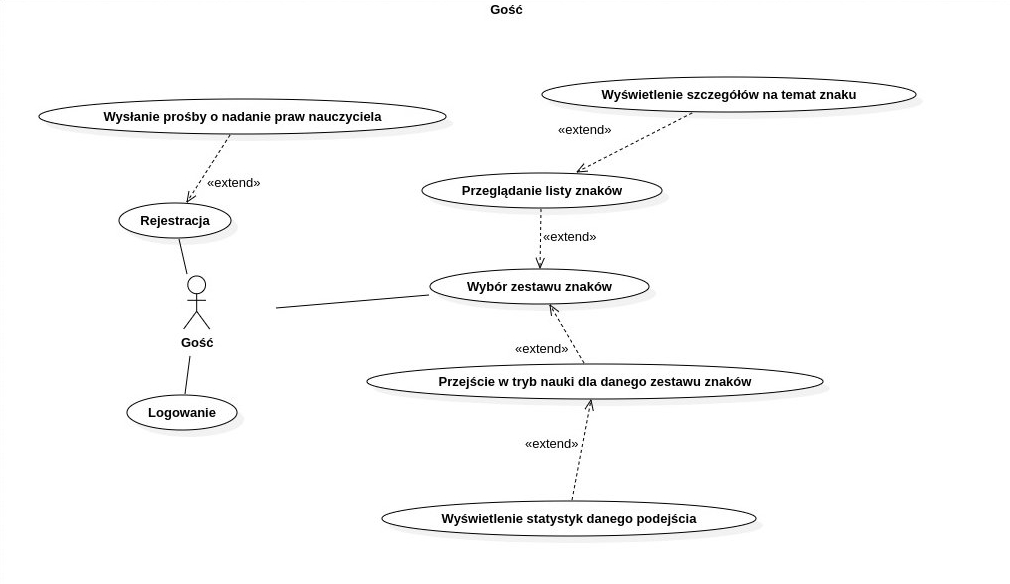
\includegraphics[width=\textwidth]{Gość}
\caption{Podpis rysunku zawsze pod rysunkiem.}
\label{fig:etykieta-rysunku}
\end{figure}
\item opis narzędzi, metod eksperymentalnych, metod modelowania itp.
\item metodyka pracy nad projektowaniem i implementacją -- dla prac, w których ma to zastosowanie
\end{itemize}


% TODO
\chapter{[Właściwy dla kierunku -- np. Specyfikacja zewnętrzna]}
\label{ch:04}

Jeśli „Specyfikacja zewnętrzna”:
\begin{itemize}
\item  wymagania sprzętowe i programowe
\item  sposób instalacji
\item  sposób aktywacji
\item  kategorie użytkowników
\item  sposób obsługi
\item  administracja systemem
\item  kwestie bezpieczeństwa
\item  przykład działania
\item  scenariusze korzystania z systemu (ilustrowane zrzutami z ekranu lub generowanymi dokumentami)
\end{itemize}

%%%%%%%%%%%%%%%%%%%%%
%% RYSUNEK Z PLIKU
%
%\begin{figure}
%\centering
%
\includegraphics[width=0.5\textwidth]{./politechnika_sl_logo_bw_pion_pl.pdf}
%\caption{Podpis rysunku zawsze pod rysunkiem.}
%\label{fig:etykieta-rysunku}
%\end{figure}
%Rys. \ref{fig:etykieta-rysunku} przestawia …
%%%%%%%%%%%%%%%%%%%%%
%
%%%%%%%%%%%%%%%%%%%%%
%% WIELE RYSUNKÓW 
%
%\begin{figure}
%\centering
%\begin{subfigure}{0.4\textwidth}
%    
\includegraphics[width=\textwidth]{./politechnika_sl_logo_bw_pion_pl.pdf}
%    \caption{Lewy górny rysunek.}
%    \label{fig:lewy-gorny}
%\end{subfigure}
%\hfill
%\begin{subfigure}{0.4\textwidth}
%    
\includegraphics[width=\textwidth]{./politechnika_sl_logo_bw_pion_pl.pdf}
%    \caption{Prawy górny rysunek.}
%    \label{fig:prawy-gorny}
%\end{subfigure}
%
%\begin{subfigure}{0.4\textwidth}
%    
\includegraphics[width=\textwidth]{./politechnika_sl_logo_bw_pion_pl.pdf}
%    \caption{Lewy dolny rysunek.}
%    \label{fig:lewy-dolny}
%\end{subfigure}
%\hfill
%\begin{subfigure}{0.4\textwidth}
%    
\includegraphics[width=\textwidth]{./politechnika_sl_logo_bw_pion_pl.pdf}
%    \caption{Prawy dolny rysunek.}
%    \label{fig:prawy-dolny}
%\end{subfigure}
%        
%\caption{Wspólny podpis kilku rysunków.}
%\label{fig:wiele-rysunkow}
%\end{figure}
%Rys. \ref{fig:wiele-rysunkow} przestawia wiele ważnych informacji, np. rys. \ref{fig:prawy-gorny} jest na prawo u góry.
%%%%%%%%%%%%%%%%%%%%%


 
\begin{figure}
\centering
\begin{tikzpicture}
\begin{axis}[
    y tick label style={
        /pgf/number format/.cd,
            fixed,   % po zakomentowaniu os rzednych jest indeksowana wykladniczo
            fixed zerofill, % 1.0 zamiast 1
            precision=1,
        /tikz/.cd
    },
    x tick label style={
        /pgf/number format/.cd,
            fixed,
            fixed zerofill,
            precision=2,
        /tikz/.cd
    }
]
\addplot [domain=0.0:0.1] {rnd};
\end{axis} 
\end{tikzpicture}
\caption{Podpis rysunku po rysunkiem.}
\label{fig:2}
\end{figure}



% TODO
\chapter{[Właściwy dla kierunku -- np. Specyfikacja wewnętrzna]}
\label{ch:05}


Jeśli „Specyfikacja wewnętrzna”:
\begin{itemize}
\item przedstawienie idei
\item architektura systemu
\item opis struktur danych (i organizacji baz danych)
\item komponenty, moduły, biblioteki, przegląd ważniejszych klas (jeśli występują)
\item przegląd ważniejszych algorytmów (jeśli występują)
\item szczegóły implementacji wybranych fragmentów, zastosowane wzorce projektowe
\item diagramy UML
\end{itemize}

% % % % % % % % % % % % % % % % % % % % % % % % % % % % % % % % % % % 
% Pakiet minted wymaga importu: \usepackage{minted}                 %
% i specjalnego kompilowania:                                       %
% pdflatex -shell-escape main                                       %
% % % % % % % % % % % % % % % % % % % % % % % % % % % % % % % % % % % 


Krótka wstawka kodu w linii tekstu jest możliwa, np.  \lstinline|int a;| (biblioteka \texttt{listings})% lub  \mintinline{C++}|int a;| (biblioteka \texttt{minted})
. 
Dłuższe fragmenty lepiej jest umieszczać jako rysunek, np. kod na rys \ref{fig:pseudokod:listings}% i rys. \ref{fig:pseudokod:minted}
, a naprawdę długie fragmenty – w załączniku.


\begin{figure}
\centering
\begin{lstlisting}
class test : public basic
{
    public:
      test (int a);
      friend std::ostream operator<<(std::ostream & s, 
                                     const test & t);
    protected:
      int _a;  
      
};
\end{lstlisting}
\caption{Pseudokod w \texttt{listings}.}
\label{fig:pseudokod:listings}
\end{figure}

%\begin{figure}
%\centering
%\begin{minted}[linenos,frame=lines]{c++}
%class test : public basic
%{
%    public:
%      test (int a);
%      friend std::ostream operator<<(std::ostream & s, 
%                                     const test & t);
%    protected:
%      int _a;  
%      
%};
%\end{minted}
%\caption{Pseudokod w \texttt{minted}.}
%\label{fig:pseudokod:minted}
%\end{figure}




% TODO
\chapter{Weryfikacja i walidacja}
\label{ch:06}
\begin{itemize}
\item sposób testowania w ramach pracy (np. odniesienie do modelu V)
\item organizacja eksperymentów
\item przypadki testowe zakres testowania (pełny/niepełny)
\item wykryte i usunięte błędy
\item opcjonalnie wyniki badań eksperymentalnych
\end{itemize}

\begin{table}
\centering
\caption{Nagłówek tabeli jest nad tabelą.}
\label{id:tab:wyniki}
\begin{tabular}{rrrrrrrr}
\toprule
	         &                                     \multicolumn{7}{c}{metoda}                                      \\
	         \cmidrule{2-8}
	         &         &         &        \multicolumn{3}{c}{alg. 3}        & \multicolumn{2}{c}{alg. 4, $\gamma = 2$} \\
	         \cmidrule(r){4-6}\cmidrule(r){7-8}
	$\zeta$ &     alg. 1 &   alg. 2 & $\alpha= 1.5$ & $\alpha= 2$ & $\alpha= 3$ &   $\beta = 0.1$  &   $\beta = -0.1$ \\
\midrule
	       0 &  8.3250 & 1.45305 &       7.5791 &    14.8517 &    20.0028 & 1.16396 &                       1.1365 \\
	       5 &  0.6111 & 2.27126 &       6.9952 &    13.8560 &    18.6064 & 1.18659 &                       1.1630 \\
	      10 & 11.6126 & 2.69218 &       6.2520 &    12.5202 &    16.8278 & 1.23180 &                       1.2045 \\
	      15 &  0.5665 & 2.95046 &       5.7753 &    11.4588 &    15.4837 & 1.25131 &                       1.2614 \\
	      20 & 15.8728 & 3.07225 &       5.3071 &    10.3935 &    13.8738 & 1.25307 &                       1.2217 \\
	      25 &  0.9791 & 3.19034 &       5.4575 &     9.9533 &    13.0721 & 1.27104 &                       1.2640 \\
	      30 &  2.0228 & 3.27474 &       5.7461 &     9.7164 &    12.2637 & 1.33404 &                       1.3209 \\
	      35 & 13.4210 & 3.36086 &       6.6735 &    10.0442 &    12.0270 & 1.35385 &                       1.3059 \\
	      40 & 13.2226 & 3.36420 &       7.7248 &    10.4495 &    12.0379 & 1.34919 &                       1.2768 \\
	      45 & 12.8445 & 3.47436 &       8.5539 &    10.8552 &    12.2773 & 1.42303 &                       1.4362 \\
	      50 & 12.9245 & 3.58228 &       9.2702 &    11.2183 &    12.3990 & 1.40922 &                       1.3724 \\
\bottomrule
\end{tabular}
\end{table}  



% TODO
\chapter{Podsumowanie i wnioski}
\begin{itemize}
\item uzyskane wyniki w świetle postawionych celów i zdefiniowanych wyżej wymagań
\item kierunki ewentualnych danych prac (rozbudowa funkcjonalna …)
\item problemy napotkane w trakcie pracy
\end{itemize}



\backmatter

%\bibliographystyle{plplain}  % bibtex
%\bibliography{biblio} % bibtex
\printbibliography           % biblatex
\addcontentsline{toc}{chapter}{Bibliografia}

\begin{appendices}

% TODO
\chapter{Spis skrótów i symboli}

\begin{itemize}
\item[DNA] kwas deoksyrybonukleinowy (ang. \english{deoxyribonucleic acid})
\item[MVC] model -- widok -- kontroler (ang. \english{model--view--controller}) 
\item[$N$] liczebność zbioru danych
\item[$\mu$] stopnień przyleżności do zbioru
\item[$\mathbb{E}$] zbiór krawędzi grafu
\item[$\mathcal{L}$] transformata Laplace'a 
\end{itemize}


% TODO
\chapter{Źródła}

Jeżeli w pracy konieczne jest umieszczenie długich fragmentów kodu źródłowego, należy je przenieść w to miejsce.

\begin{lstlisting}
if (_nClusters < 1)
	throw std::string ("unknown number of clusters");
if (_nIterations < 1 and _epsilon < 0)
	throw std::string ("You should set a maximal number of iteration or minimal difference -- epsilon.");
if (_nIterations > 0 and _epsilon > 0)
	throw std::string ("Both number of iterations and minimal epsilon set -- you should set either number of iterations or minimal epsilon.");
\end{lstlisting}


% % % % % % % % % % % % % % % % % % % % % % % % % % % % % % % % % % % 
% Pakiet minted wymaga odkomentowania w pliku config/settings.tex   %
% importu pakietu minted: \usepackage{minted}                       %
% i specjalnego kompilowania:                                       %
% pdflatex -shell-escape praca                                      %
% % % % % % % % % % % % % % % % % % % % % % % % % % % % % % % % % % % 

%\begin{minted}[linenos,breaklines,frame=lines]{c++}
%if (_nClusters < 1)
%   throw std::string ("unknown number of clusters");
%if (_nIterations < 1 and _epsilon < 0)
%   throw std::string ("You should set a maximal number of iteration or minimal difference -- epsilon.");
%if (_nIterations > 0 and _epsilon > 0)
%   throw std::string ("Both number of iterations and minimal epsilon set -- you should set either number of iterations or minimal epsilon.");
%\end{minted}


% TODO
\chapter{Lista dodatkowych plików, uzupełniających tekst pracy} 


W systemie do pracy dołączono dodatkowe pliki zawierające:
\begin{itemize}
\item źródła programu,
\item dane testowe,
\item film pokazujący działanie opracowanego oprogramowania lub zaprojektowanego i~wykonanego urządzenia,
\item itp.
\end{itemize}


\listoffigures
\addcontentsline{toc}{chapter}{Spis rysunków}
\listoftables
\addcontentsline{toc}{chapter}{Spis tabel}

\end{appendices}

\end{document}


%% Finis coronat opus.

